\begin{tframe}{Pipeline}

\bigskip
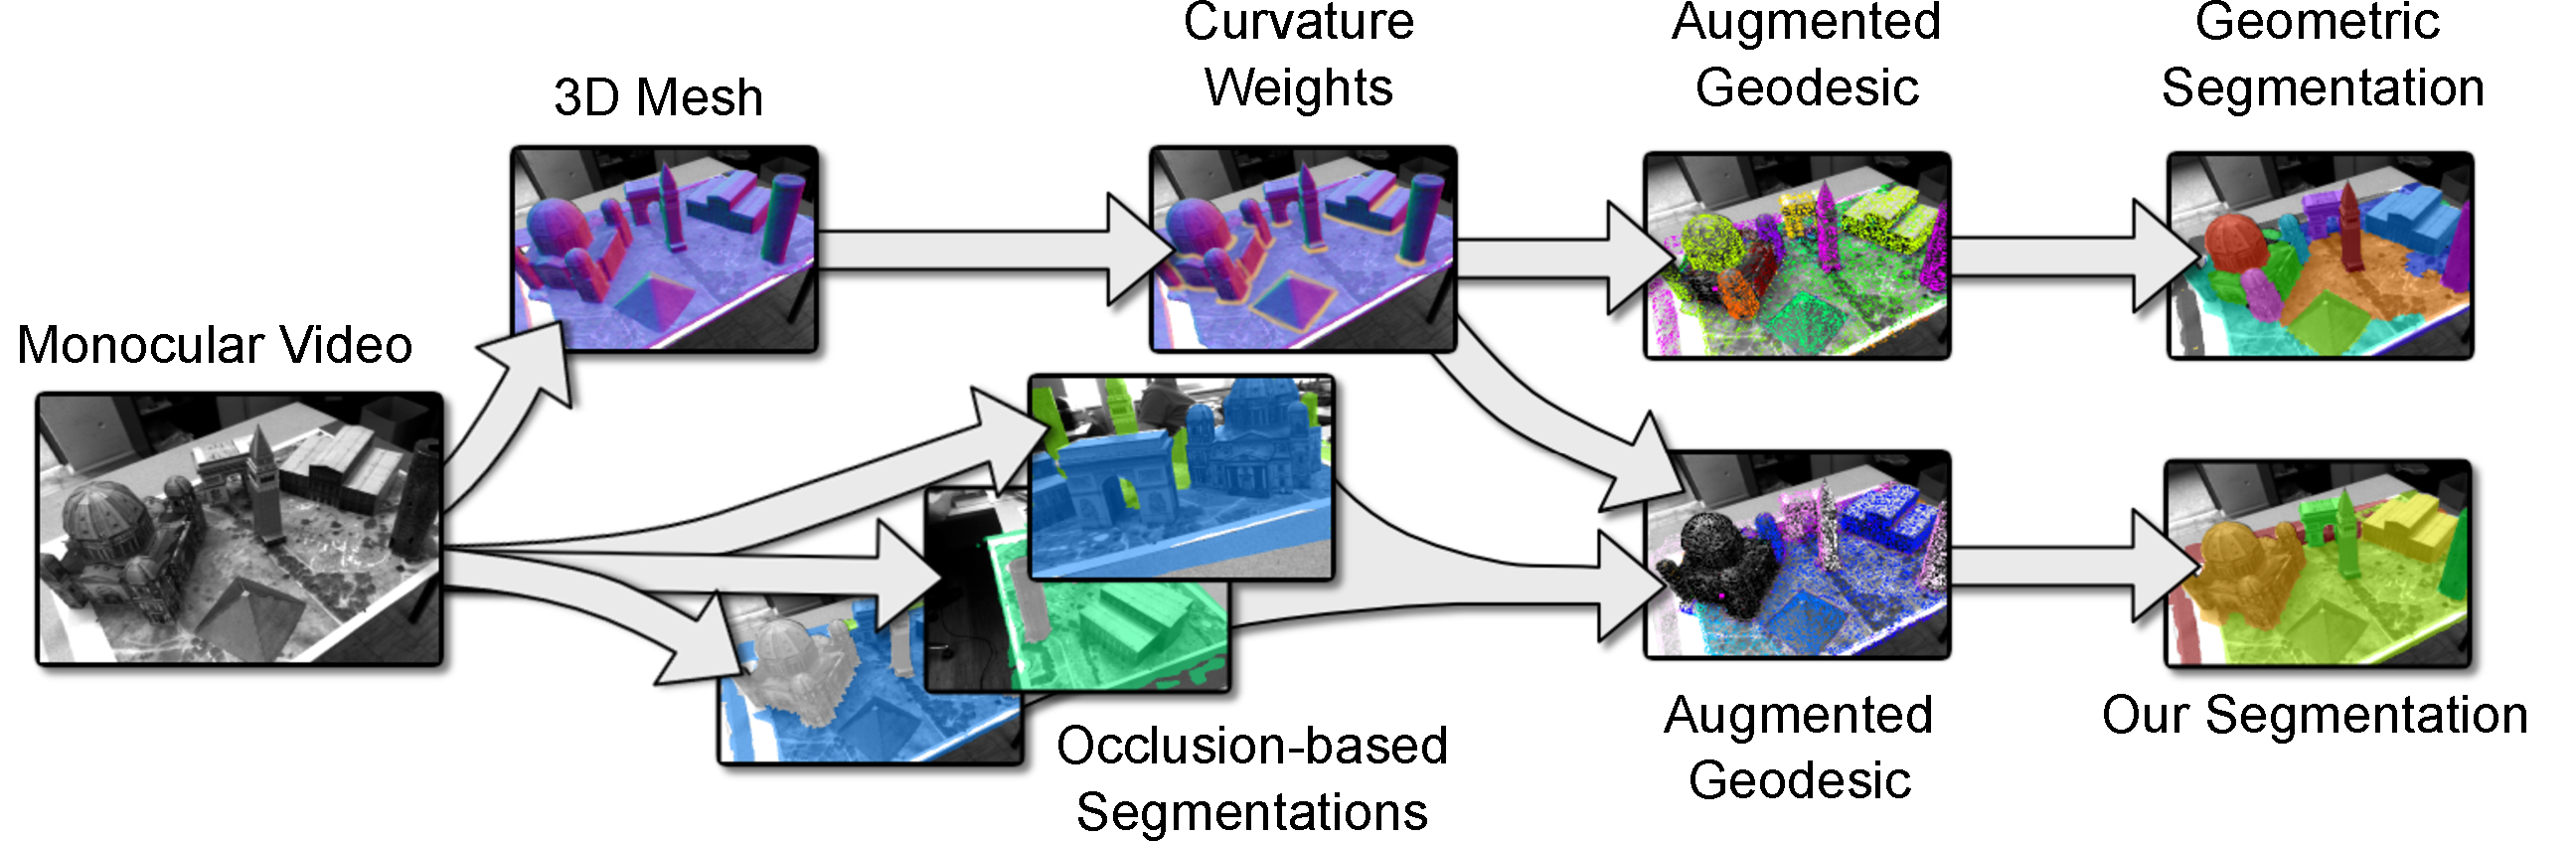
\includegraphics[width=4in]{media_solobj/pipeline}
\end{tframe}

\begin{tframe}{VIDEO}
\end{tframe}

\begin{tframe}{Comparisons}
\resizebox{.9\textwidth}{!}{
\begin{tabularx}{8in}{r *{4}{cc}}
\toprule
& \multicolumn{2}{c}{\emph{City of Sights}}
& \multicolumn{2}{c}{\emph{Pipes1}}
& \multicolumn{2}{c}{\emph{Pipes2}}
& \multicolumn{2}{c}{\emph{Tree}}\\
& Frame & Scene & Frame & Scene & Frame & Scene & Frame & Scene\\
\cmidrule(lr){2-3} \cmidrule(lr){4-5} \cmidrule(lr){6-7} \cmidrule(lr){8-9}
CGAL
\footnote{ L. Shapira, A. Shamir, and D. Cohen-Or. Consistent mesh
partitioning and skeletonisation using the shape diameter
function. \emph{Vis. Comput.}, 24(4):249–259, Mar. 2008} 
\begin{tabular}{r} F-Score \\ Precision \\ Recall \end{tabular} & 
\begin{tabular}{c} $.803\pm.041$ \\ $.822\pm.043$ \\ $.785\pm.041$ \end{tabular} & 
\begin{tabular}{c} .787 \\ .798 \\ .776 \end{tabular} &

\multicolumn{2}{c}{Fails} &

\begin{tabular}{c} ${\bm{.915\pm.032}}$ \\ $.959\pm.036$ \\ $.875\pm.041$ \end{tabular} &
\begin{tabular}{c} ${\bm{.869}}$ \\ .903 \\ .838 \end{tabular} &

\begin{tabular}{c} $.643\pm.049$ \\ $.633\pm.058$ \\ $.657\pm.053$ \end{tabular} &
\begin{tabular}{c} .604 \\ .608 \\ .599 \end{tabular}\\
\midrule

WCSeg
\footnote{O. van Kaick, N. Fish, Y. Kleiman, S. Asafi.
Shape segmentation by approximate convexity analysis.
\emph{ACM Trans. on Graphics, 2014}.}
\begin{tabular}{r} F \\ P \\ R \end{tabular} & 
\begin{tabular}{c} $.775\pm.028$ \\ $.938\pm.033$ \\ $.661\pm.033$ \end{tabular} & 
\begin{tabular}{c} .732 \\ .912 \\ .612 \end{tabular} &

\begin{tabular}{c} ${\bm{.730\pm.030}}$ \\ $.843\pm.040$ \\ $.645\pm.036$ \end{tabular} & 
\begin{tabular}{c} ${\bm{.725}}$ \\ .841 \\ .637 \end{tabular} &

\begin{tabular}{c} $.738\pm.045$ \\ $.820\pm.050$ \\ $.676\pm.068$ \end{tabular} &
\begin{tabular}{c} .730 \\ .904 \\ .612 \end{tabular} &

\begin{tabular}{c} $.806\pm.027$ \\ $.885\pm.031$ \\ $.742\pm.038$ \end{tabular} &
\begin{tabular}{c} .747 \\ .889 \\ .644 \end{tabular}\\
\midrule

\begin{tabular}{c} Ours \\ (Geom. only) \end{tabular} \begin{tabular}{r} F \\ P \\ R \end{tabular} & 
\begin{tabular}{c} ${\bm{.923\pm.018}}$ \\ $.986\pm.018$ \\ $.867\pm.020$ \end{tabular} & 
\begin{tabular}{c} ${\bm{.788}}$ \\ .866 \\ .722 \end{tabular} &

\begin{tabular}{c} $.705\pm.036$ \\ $.761\pm.043$ \\ $.658\pm.040$ \end{tabular} & 
\begin{tabular}{c} .648 \\ .690 \\ .612 \end{tabular} &

\begin{tabular}{c} $.818\pm.045$ \\ $.820\pm.056$ \\ $.818\pm.047$ \end{tabular} &
\begin{tabular}{c} .701 \\ .751 \\ .657 \end{tabular} &

\begin{tabular}{c} $.720\pm.036$ \\ $.763\pm.036$ \\ $.683\pm.041$ \end{tabular} &
\begin{tabular}{c} .729 \\ .783 \\ .681 \end{tabular}\\
\midrule

\begin{tabular}{c} Ours \\ (Geom. + Vis.) \end{tabular} \begin{tabular}{r} F \\ P \\ R \end{tabular} & 
\begin{tabular}{c} $.870\pm.043$ \\ $.853\pm.028$ \\ $.888\pm.062$ \end{tabular} & 
\begin{tabular}{c} .767 \\ .763 \\ .770 \end{tabular} &

\begin{tabular}{c} $.662\pm.027$ \\ $.689\pm.040$ \\ $.637\pm.030$ \end{tabular} & 
\begin{tabular}{c} .605 \\ .611 \\ .599 \end{tabular} &

\begin{tabular}{c} $.804\pm.063$ \\ $.810\pm.064$ \\ $.800\pm.072$ \end{tabular} &
\begin{tabular}{c} .648 \\ .679 \\ .620 \end{tabular} &

\begin{tabular}{c} ${\bm{.828\pm.034}}$ \\ $.803\pm.028$ \\ $.856\pm.032$ \end{tabular} &
\begin{tabular}{c} ${\bm{.836}}$ \\ .790 \\ .888 \end{tabular}\\
\midrule

\end{tabularx}}
\end{tframe}


\begin{tframe}{Contribution}
\begin{itemize}
 \item First bounds on indistinguishable set with IMU bias drift.
 \item Developed system for video segmentation leveraging image-plane segmentations.
\end{itemize}
\end{tframe}